% documentclass
% set font size=11 (11pt)
% set paper format=A4 (a4paper)
% set equation alignment to left (fleqn)
\documentclass[11pt,a4paper,fleqn]{article}


% Preamble
% use the inputenc and fontenc packages to use French accents
\usepackage[utf8]{inputenc}
\usepackage[T1]{fontenc}
% allow for arbitrary font size
\usepackage{anyfontsize}
% set the font as Time New Roman (the Latex equivalent, at least)
% \usepackage{mathptmx}
% set the size of the document margins using the geometry package
\usepackage[lmargin=0.97in,rmargin=0.97in,tmargin=1.4in,bmargin=1.4in]{geometry}
% turn the color of footnote markers to black
\renewcommand\thefootnote{\textcolor{black}{\arabic{footnote}}}
% suppress indents on footnotes
\usepackage[hang,flushmargin]{footmisc}
% automatically generates colored brackets around references
\usepackage{fncylab} \labelformat{equation}{(#1)}
% supress indent on new paragraphs
\setlength{\parindent}{0pt}
% use the amsmath package to include mathematical symbols
\usepackage{amsmath}
% suppress the space between the left margin and the equations (fleqn still leaves some space by default)
\setlength{\mathindent}{0pt}
% create a new environment to left flush the equation with the align environment
\makeatletter
\newenvironment{lflalign}{ \vspace{-3mm}%
  \def\align@preamble{%
    &\strut@
    \setboxz@h{\@lign$\m@th\displaystyle{####}$}%
    \ifmeasuring@\savefieldlength@\fi
    \set@field
    \hfil
    \tabskip\z@skip
    &\setboxz@h{\@lign$\m@th\displaystyle{{}####}$}%
    \ifmeasuring@\savefieldlength@\fi
    \set@field
    \hfil
    \tabskip\alignsep@
  }
  \flalign}
{\endflalign}
\makeatother
% use the ammssymb package to use mathematical symbols
\usepackage{amssymb}
% create new commands for mathematical symbols
\DeclareMathOperator{\N}{\mathbb{N}}
\DeclareMathOperator{\Z}{\mathbb{Z}}
\DeclareMathOperator{\Q}{\mathbb{Q}}
\DeclareMathOperator{\R}{\mathbb{R}}
\DeclareMathOperator{\Pb}{\mathbb{P}}
% declare the cmsy (computer modern symbol) math alphabet to define appropriate fonts for the U and N mathematical symbols
\DeclareMathAlphabet\mathbcal{OMS}{cmsy}{m}{n}
% create new commands for mathematical symbols
\DeclareMathOperator{\E}{\mathbcal{E}}
\DeclareMathOperator{\Ex}{\mathbb{E}}
\DeclareMathOperator{\F}{\mathbcal{F}}
\DeclareMathOperator{\G}{\mathbcal{G}}
\DeclareMathOperator{\M}{\mathbcal{M}}
\DeclareMathOperator{\HH}{\mathbcal{H}}
\DeclareMathOperator{\QQ}{\mathbcal{Q}}
\DeclareMathOperator{\PP}{\mathbcal{P}}
\DeclareMathOperator{\Noo}{\mathbcal{N}}
\DeclareMathOperator{\U}{\mathbcal{U}}
% use the bbm package to be able to use the double stroke 1 for the indicator function
\usepackage{bbm}
\DeclareMathOperator{\ind}{\mathbbmss{1}}
% use the bm package to use bold characters in math mode
\usepackage{bm}
% create a new command for black square bullets
\newcommand{\bs}{\scalebox{0.7}{$\blacksquare$} \hspace{2mm}}
% use the relsize package to be abe to change the size of mathematical symbols
\usepackage{relsize}
% define a new command for in-line small summation
\newcommand{\ssumm}[2]{\underset{\scriptscriptstyle #1}{\overset{\scriptscriptstyle #2}{\mathlarger{\mathlarger{\mathlarger{\Sigma}}}}} \hspace{0.5mm}}
% define a new command for in-line small products
\newcommand{\sprod}[2]{\underset{\scriptscriptstyle #1}{\overset{\scriptscriptstyle #2}{\mathlarger{\mathlarger{\mathlarger{\Pi}}}}} \hspace{0.5mm}}
% Use the caption package to customize captions (titles) of tables and graphs
\usepackage[font=small,labelfont=bf]{caption}
% use float package to force figure the be positioned where indicated
\usepackage{float}
% use the graphicx package to be able to resize tables
\usepackage{graphicx}


\begin{document}

% command to check unused bibliography entries
% \nocite{*}
{\fontsize{20pt}{22pt}\selectfont \textbf{Probabilistic tools} \par}
\vspace{10mm}
Central Limit Theorem

Let $(X_n)_{n \ge 1}$ be a real and independent sequence with same law such that $\mu = \mathbb{E}[X_1]$ and \\
$\mathbb{V}[X_1]=\sigma^2$ are defined ($\mathbb{V}[X_1] \leq +\infty$). Noting $\bar{X}_n=\frac{1}{n}(X_1 + ... + X_n)$, we have:
\begin{center}
$\sqrt{n}\frac{(\bar{X}_n-\mu)}{\sigma} \sim_{n \to \infty} \mathcal{N}(0,1)$
\end{center}

\vspace{5mm}
Spectral Theorem

Let $M$ be a symmetric matrix with real coefficients. Then it exists $U$ orthogonal and $D$ diagonal with real coefficients such that $M=UDU^T$.

\vspace{5mm}
{\fontsize{20pt}{22pt}\selectfont \textbf{Inferential statistics} \par}
\vspace{10mm}
{\fontsize{12pt}{22pt} \textbf{Likelihood method}\par}

\vspace{5mm}

This method consists on finding the parameter that maximizes the likelihood of an event. It is usually done when we know the type of law of a random variable (uniform, gaussian etc.) and we are looking for the parameter that maximizes the likelihood ($\approx$ probability) that an event occurs.

\vspace{5mm}

$L(\theta; x_1,...,x_n) = \prod_{i=1}^{n}f(x_i;\theta)$ which is the product of densities across all samples.

In discrete form: $L(\theta; x_1,...,x_n) = \prod_{i=1}^{n}\mathbb{P}(X = x_i; \theta)$


\vspace{5mm}

\textit{Note (wording clarification)}: $L(\theta | X) = \mathbb{P} (X | \theta)$

$\mathbb{P} (X | \theta)$: the probability of observing an event with fixed model parameters.

$L(\theta | X)$: the likelihood of the parameters taking certain values given that we observe an event.

\vspace{5mm}

Intuitively, we want to find the $\theta$ that maximizes a certain event, that is, obtaining some data $X$ (which is why we have $X | \theta$).

We often use the log in order to get rid of power coefficients appearing with the product. \\
\textit{likelihood equation}: $\frac{d}{d\theta}ln(L(x_1,...,x_n;\theta))=0$

\vspace{5mm}

\textit{Note}: in machine learning, we use likelihood maximization in unsupervised learning when we want to estimate parameters of a distribution sample (generative models).

\vspace{5mm}
{\fontsize{20pt}{22pt}\selectfont \textbf{Exploratory statistics} \par}
\vspace{10mm}
Mahalanobis distance

Mahalanobis distance is a good alternative to Euclidean distance. For any given point $x$ in a set $X$, the squared Mahalanobis distance is:

$$D^2=(x-\mu_X)^T\Sigma^{-1}(x-\mu_X)$$

Advantage : it takes into account the data standard deviation and correlation. The more the data is dispersed, the lower the distance is. Indeed, using the inverse matrix is like if we divided the distance from the mean $(x-\mu_X)$ by the standard deviation.

\textit{Note}: Euclidean distance is when $\Sigma=Id$.

\vspace{5mm}
\vspace{10mm}
{\fontsize{20pt}{22pt}\selectfont \textbf{Predictive models} \par}
\vspace{10mm}
{\fontsize{12pt}{22pt} \textbf{ROC curve}\par}

\vspace{5mm}

ROC curve is used essentially for binary classification.

ROC = Receiver Operating Curve

\vspace{5mm}

\underline{Use of the ROC curve}

\vspace{5mm}

One model:

We use ROC curve to evaluate the performance of one classifying model that we can obtain when varying a threshold.

\vspace{5mm}

Several models:

We use ROC curve to compare several classifying models in evaluating the area under the curve (AUC) for a range of threshold.

\vspace{5mm}

\underline{Intuition}

\vspace{5mm}

After running the prediction of a specific model, we draw the confusion matrix (actual vs predited) with a certain threshold.

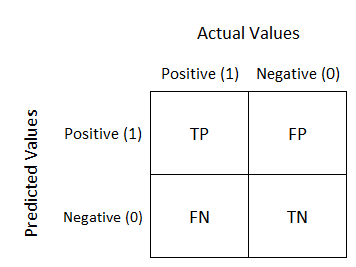
\includegraphics[scale=0.5]{../images/confusionmatrice.png}

\vspace{5mm}

We then modify the threshold and draw another confusion matrix.

The ROC graph summarizes all of the confusion matrices that each threshold produced.

\vspace{5mm}

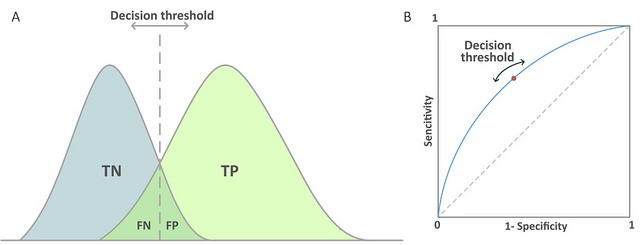
\includegraphics[scale=0.5]{../images/overlap_roc.jpeg}

\vspace{5mm}

On the left picture we see the ability of a model to give a clear distinction between the two classes. The curves are drawn from the predictions and the actual results (\textbf{how?})

\vspace{5mm}

\underline{Implementation}

\vspace{5mm}

1. Get probability predictions

2. Sort the probabilities (prediction)

3. Sort the validation (actual) according to previous sort

4. Loop on the sorted validation. At each iteration:

- increment TP or FP

- compute the TPR and FPR.

5. Plot (FPR, TPR)

\vspace{5mm}

See \textit{https://docs.eyesopen.com/toolkits/cookbook/python/plotting/roc.html} for an implementation example, or data challenge Face\_Recognition.

\vspace{5mm}

\vspace{10mm}
\end{document} 
